
\section[Service组件]{Service组件}
Service --- Android四大组件之一。

\subsection[Service的分类]{Service的分类}
Service分为两类:\par
\begin{description}
  \item[Started Service:] 通过调用startService()接口启动的Service。这种Service将“无限期”运行在后台,
                          有两种方法可以结束它:在执行过程中调用stopSelf()结束自己、别的组件调用stopService() 结束它。
  \item[Bound Service:] 通过调用bindService()接口启动的Service。在工作完成时,调用者应该调用unBindService()
                        解除绑定。没有任何绑定时,Service将自行被系统销毁。
\end{description}

\subsection[Service basic interface]{Service basic interface}
\begin{coloredenumerate}
  \item onStartCommand(): 当调用startService()时,系统将会调用到该接口,它与Started Service对应。
  \item onBind(): 当调用bindService()时,系统将会调用到该接口,它是Bound Service的启动接口。
  \item onCreate(): Service生命周期的开始,无论哪种Service,启动时都会调用该接口。
  \item onDestroy(): Service生命周期的结束,无论哪种Service,结束时都会调用到该接口。
\end{coloredenumerate}

由于started Service有可能无限期运行,所以系统资源紧张时会被kill掉,此时就需要onStartCommand()以返回值
的形式告知系统,当Service被kill的时候,系统应该如何处理它。返回值有以下几种:\par
\begin{coloredenumerate}
  \item START\_NOT\_STICKY: Service被kill掉之后,不要重新启动它,除非有Intent提交请求,推荐!
  \item START\_STICKY: Service被kill之后重新启动它,但是不要传递最后一个Intent。
  \item START\_REDELIVER\_INTENT: Service被kill之后,重新启动它并传递最后一个Intent给它。
\end{coloredenumerate}

\subsection[Started Service分类]{Started Service分类}
Started Service分类两类:\par
\begin{coloredenumerate}
  \item IntentService: 该类Service启动一个worker线程“逐个”、“顺序”处理所有的start请求。
  \item 直接继承Service类,一般用于启动多线程并发处理start请求的情况。
\end{coloredenumerate}

\subsection[Bound Service分类]{Bound Service分类}
Bound Service允许其他组件绑定到它上面并与之交互,该service必须实现onBind()函数,并返回
一个IBinder对象,该对象是Client与Service交互的接口。多个Client可以同时绑定到Service上。
实现Bound Service的关键是实现IBinder对象,根据创建IBinder对象的方式可以分为
以下几类Bound Service:\par
\begin{coloredenumerate}
  \item 继承IBinder类:Service是app的私有组件并且与Client运行在相同的进程中。
  \item 使用Messenger:Service与Client不在同一个进程中,使用Messenger实现进程间通信,
        Messenger会将多个线程的请求统一到一个消息队列中,供Service逐个处理,所以
        不用考虑Service执行代码的线程安全与否。
  \item 使用AIDL:如果希望Service能够“同时”处理多个请求,可以直接使用AIDL,此时
        Service执行代码必须是多线程的,而且要做到线程安全性。事实上,Messenger的
        底层正是AIDL。
\end{coloredenumerate}
Bound Service将放到单独的notes条目\ref{sec:boundservice}中讲解。

\subsection[Service的生命周期]{Service的生命周期}
\begin{figure}[ht]
  \centering
  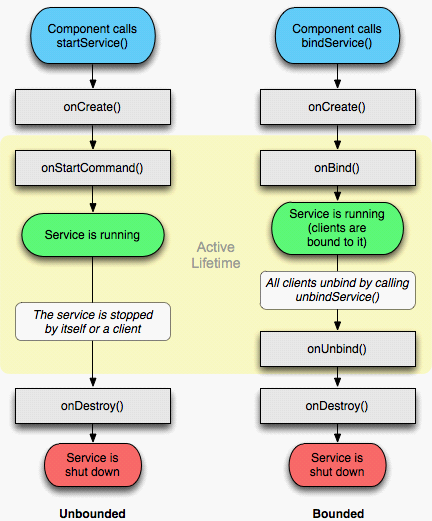
\includegraphics[width=.7\textwidth]{picturedir/life_cycle_of_service.png}\\
  \caption{Life cycle of Service}\label{fig:service}
\end{figure}
详细内容见图 \ref{fig:service}

\subsection[Service v.s. Thread]{Service v.s. Thread}
如果想要在UI线程以外执行任务,并且该任务只在用户与应用程序交互的过程中执行,
那么应该创建线程而非Service。

\subsection[service默认运行在UI线程]{service默认运行在UI线程}
这一点是如此重要,以至于用一个单独的subsection来记录它。

\section[Bound Service]{Bound Service}\label{sec:boundservice}
实现Bound Service的关键是:IBinder接口。
\subsection[使用IBinder]{使用IBinder}
\subsubsection[Service端代码]{Service端代码}
\inputminted[linenos,tabsize=4,bgcolor=srcbg]{java}{srcdir/LocalService.java}

\subsubsection[Client端代码]{Client端代码}
\inputminted[linenos,tabsize=4,bgcolor=srcbg]{java}{srcdir/BindingActivity.java}

\subsection[使用Messenger]{使用Messenger}
略。

\subsection[AIDL的使用方法]{AIDL的使用方法}
所有的代码均在Eclipse环境下运行。\par\bigskip
AndroidManifest文件:\par
\inputminted[linenos,tabsize=4,bgcolor=srcbg]{xml}{srcdir/AIDLManifest.xml}

\subsubsection[Server端代码]{Server端代码}
AIDL service的aidl文件:\par
\begin{javacode}
/* IAIDLServerService.aidl */
package com.example.aidldemo.server;

import com.example.aidldemo.server.Book;

interface IAIDLServerService {
  String sayHello();
  Book getBook();
}
\end{javacode}

Book类的aidl文件:\par
\begin{javacode}
/* IBook.aidl */
parcelable Book;
\end{javacode}

Service代码:\par
\inputminted[linenos,tabsize=4,bgcolor=srcbg]{java}{srcdir/AIDLServerService.java}

Book类代码:\par
\inputminted[linenos,tabsize=4,bgcolor=srcbg]{java}{srcdir/Book.java}

\subsubsection[Client端代码]{Client端代码}
Client端代码,结果将在Logcat中打印出来:\par
\inputminted[linenos,tabsize=4,bgcolor=srcbg]{java}{srcdir/ClientActivity.java}

\subsubsection[输出结果]{输出结果}
\begin{bashcode}
D/ClientActivity(10184): book name: Android Notes, book price: 42
\end{bashcode}